\section{Rozšírenie predošlej práce}

\begin{figure*}
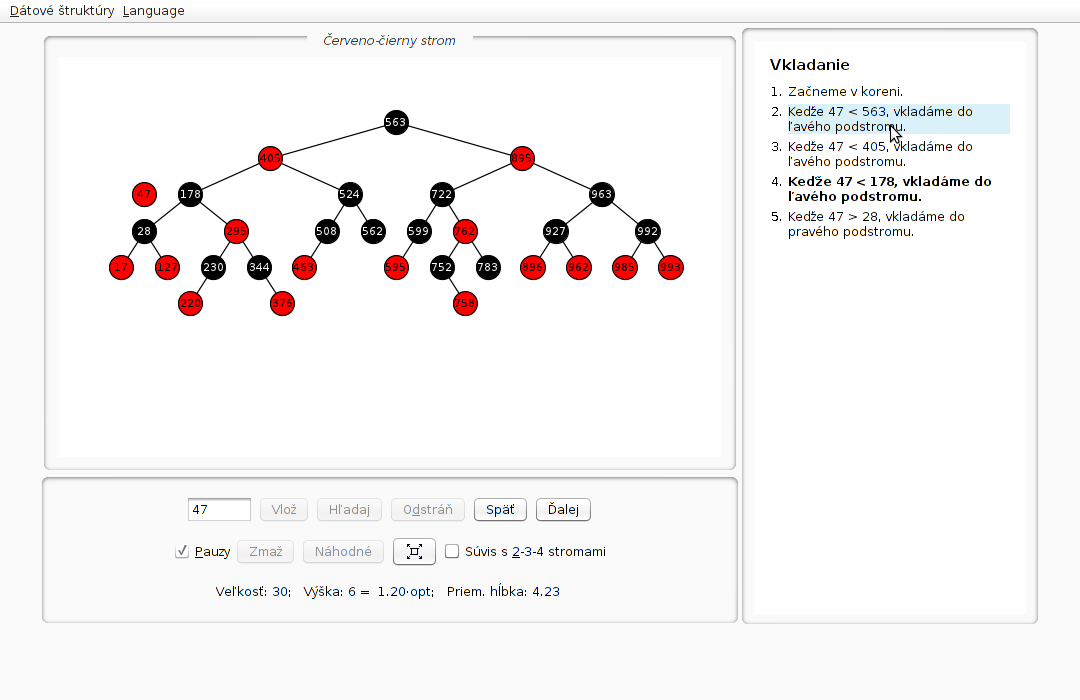
\includegraphics[width=2\columnwidth]{obrazky/historia.png}
\caption{\emph{Softvér Gnarley Trees.} Vpravo je história krokov. V histórií 
sa dá navigovať buď pomocou tlačidiel \uv{Späť}/\uv{Ďalej}, alebo kliknutím na 
konkrétny krok v histórií.}
\label{img:historia} 
\end{figure*}

Projekt Gnarley Trees sme rozšírili nielen o vizualizácie ďalších dátových
štruktúr, ale pribudli aj softvérové (vizualizačné) vylepšenia:
kompaktnejšie vykresľovanie stromov, história krokov s možnosťou návratu,
či približovanie a vzďaľovanie.

\subsection{Tesnejšie vykresľovanie stromov}

V pôvodnej verzii programu sa stromy vykresľovali tak, že vertikálna súradnica 
predstavovala hĺbku v strome a horizontálna poradie vrcholu v \emph{
inorderovom prechode} stromu. Tento jednoduchý spôsob však nešetrí priestor
a pri štruktúrach ako union-find či písmenkový strom by výsledné stromy 
vyzerali škaredo. Preto sme sa rozhodli pre stromy implementovať 
alternatívny spôsob rozloženia, ktorý pre binárne stromy navrhli \citet{reingold}
a na všeobecné stromy rozšíril \citet{walker}. Tieto rozloženia vykresľujú
vrcholy stromov čo najtesnejšie, pričom dodržujú tieto estetické pravidlá: 
\begin{itemize} 
\item vrcholy v rovnakej hĺbke sú vykreslené na jednej priamke a priamky 
určujúce jednotlivé úrovne sú rovnobežné; 
\item poradie synov je zachované; 
\item otec leží v strede nad najľavejším a najpravejším synom; 
\item izomorfné podstromy sa vykreslia identicky až na presunutie;
\item ak vo všetkých vrcholoch obrátime poradie všetkých synov, výsledný strom 
sa vykreslí zrkadlovo.
\end{itemize}
Reingoldov-Tilfordov, aj zovšeobecnený Walkerov algoritmus pracuje v lineárnom
čase.
